% =====================================================================
%  How Many Demonstrations Does a €400 Robot Arm Need?
%  Public project report — SO-101 / LeRobot / ACT
%  Compile with: tectonic -X compile so101_report_EN.tex
%  Figures: python scripts/make_report_figures.py (see Appendix A)
% =====================================================================
\documentclass[11pt,a4paper]{article}

\usepackage[english]{babel}
\usepackage{libertinus}
\usepackage{microtype}

\usepackage[margin=2.3cm,top=2cm]{geometry}
\usepackage{graphicx}
\graphicspath{{figures/}}
\usepackage{booktabs}
\usepackage{array}
\usepackage{tabularx}
\usepackage{listings}
\usepackage[table]{xcolor}
\usepackage{enumitem}
\usepackage[compact,small]{titlesec}
\usepackage[font=small,labelfont=bf,margin=0pt,skip=4pt]{caption}
\usepackage{qrcode}
\usepackage[most]{tcolorbox}
\usepackage{etoolbox}
\usepackage[section]{placeins}

\definecolor{accent}{HTML}{2A78D6}
\definecolor{ink2}{HTML}{52514E}
\definecolor{codebg}{RGB}{246,246,246}
\definecolor{boxbg}{HTML}{F4F7FB}
% outcome scale (same colours as the figures)
\definecolor{outA}{HTML}{1D5FAE}
\definecolor{outB}{HTML}{5B9BE3}
\definecolor{outC}{HTML}{A9C9EF}
\definecolor{outD}{HTML}{E4E3DF}

\usepackage[colorlinks,linkcolor=accent,urlcolor=accent,citecolor=accent]{hyperref}
\hypersetup{
  pdftitle={How Many Demonstrations Does a €400 Robot Arm Need?},
  pdfauthor={Fabio Bariletti},
  pdfsubject={Data efficiency and failure analysis of ACT imitation learning on the SO-101 arm},
  pdfkeywords={imitation learning, behaviour cloning, ACT, LeRobot, SO-101, robotics}
}

\setlist{nosep,leftmargin=1.4em}
\setlength{\parskip}{0.35em}
\setlength{\parindent}{0pt}
\tolerance=1500
\setlength{\emergencystretch}{3em}

\lstdefinestyle{sh}{
  backgroundcolor=\color{codebg},
  basicstyle=\ttfamily\scriptsize,
  breaklines=true,
  columns=fullflexible,
  frame=single,
  framesep=4pt,
  rulecolor=\color{gray!35},
  showstringspaces=false,
  language=bash,
  xleftmargin=0pt
}
\lstset{style=sh}

% ---------------------------------------------------------------------
%  LINKS — fill these in; empty ones render as "link coming soon"
% ---------------------------------------------------------------------
\newcommand{\urlRepo}{https://github.com/FabioBariletti/so101-data-efficiency}  % GitHub repository
\newcommand{\urlOverview}{}    % video: project overview / teleoperation
\newcommand{\urlSuccess}{}     % video: successful rollout
\newcommand{\urlFailure}{}     % video: near miss
\newcommand{\urlRetry}{}       % video: miss, correction, success (firstFail_thenSucc)
\newcommand{\urlHF}{https://huggingface.co/Fabyo04}

% thumbnail + title + (QR code and link | placeholder)
\newcommand{\videocard}[3]{%
  \begin{minipage}[t]{0.235\textwidth}\centering
    \ifdefempty{#3}{\includegraphics[width=\linewidth]{#1}}%
      {\href{#3}{\includegraphics[width=\linewidth]{#1}}}\\[3pt]
    {\footnotesize\textbf{#2}}\\[2pt]
    \ifdefempty{#3}{{\scriptsize\color{ink2}link coming soon}}%
      {\qrcode[height=1.1cm]{#3}\\[1pt]{\scriptsize\href{#3}{watch video}}}
  \end{minipage}}

% inline link that degrades gracefully when the URL is still empty
\newcommand{\linkor}[2]{\ifdefempty{#1}{#2 \textcolor{ink2}{(coming soon)}}{\href{#1}{#2}}}

% evaluation outcome cells
\newcommand{\oa}{\cellcolor{outA}\textcolor{white}{\textbf{a}}}
\newcommand{\ob}{\cellcolor{outB}\textcolor{white}{\textbf{b}}}
\newcommand{\oc}{\cellcolor{outC}c}
\newcommand{\od}{\cellcolor{outD}\textcolor{ink2}{d}}

\begin{document}

% =====================================================================
%  TITLE BLOCK
% =====================================================================
\begin{center}
  {\LARGE\bfseries How Many Demonstrations Does a €400 Robot Arm Need?}\\[6pt]
  {\large Low training loss, low task success: diagnosing a perceptual bottleneck\\
  in imitation learning on the SO-101 arm}\\[10pt]
  {\normalsize Fabio Bariletti}\\[1pt]
  {\small\color{ink2} MSc Artificial Intelligence Systems \quad·\quad July -- October 2026}\\[4pt]
  {\small \linkor{\urlRepo}{Code} \quad·\quad \href{\urlHF}{Datasets \& models}
   \quad·\quad \hyperref[sec:videos]{Videos}}
\end{center}

\vspace{2pt}
\begin{figure}[h]
  \centering
  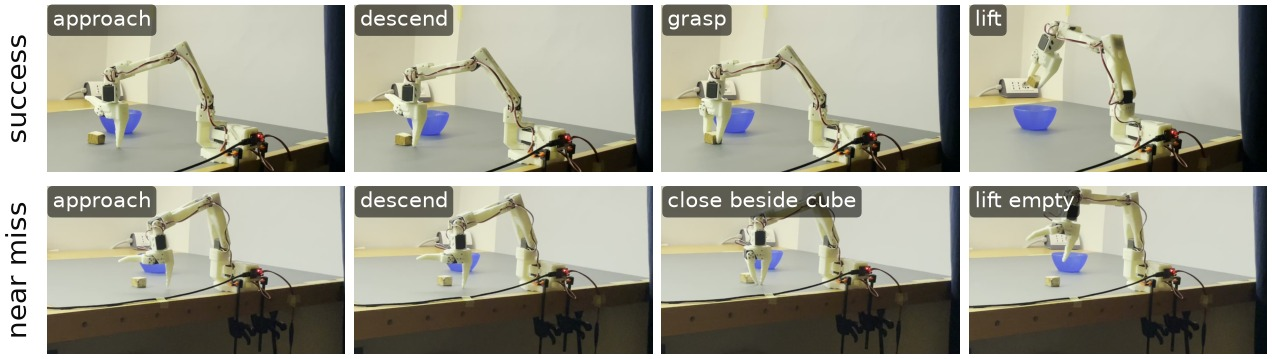
\includegraphics[width=\textwidth]{rollouts.jpg}
  \caption{Autonomous rollouts of ACT policies trained on setup-2 data.
  \textbf{Top:} success (\texttt{v2\_100}).
  \textbf{Bottom:} the characteristic failure, a \emph{near miss}
  (\texttt{v2\_024}) --- the policy
  executes a well-formed grasp in the right place, but closes within about a
  centimetre of the cube and lifts an empty gripper.}
  \label{fig:teaser}
\end{figure}

\begin{tcolorbox}[enhanced,colback=boxbg,colframe=boxbg,boxrule=0pt,arc=2pt,
  left=8pt,right=8pt,top=5pt,bottom=5pt]
\small
\begin{tabularx}{\linewidth}{@{}>{\raggedright\arraybackslash}X@{\hspace{12pt}}>{\raggedright\arraybackslash}X@{\hspace{12pt}}>{\raggedright\arraybackslash}X@{}}
{\Large\bfseries\color{accent} 4$\times$ data}\newline
24\,$\rightarrow$\,100 demonstrations: success 1/15\,$\rightarrow$\,2/15, \textbf{no detectable gain}
&
{\Large\bfseries\color{accent} $\approx$1\,cm}\newline
8--12 of 15 rollouts per model are \textbf{near misses}: right motion, gripper closes next to the cube
&
{\Large\bfseries\color{accent} Likely cause}\newline
at the grasp, neither camera shows gripper and cube together: the limit appears \textbf{perceptual} rather than data-related
\end{tabularx}
\end{tcolorbox}

\begin{abstract}
\noindent
I built an SO-101 robot arm from parts, recorded three datasets of teleoperated
demonstrations across two camera setups, trained four ACT policies, and
evaluated three of them on a pick-and-place task under a protocol fixed in
advance. \textbf{The headline result is negative, and the interesting part is
why.} All policies converge in training (final $L_1$ loss 0.05--0.09, an order
of magnitude below its initial value) but succeed on only 7--13\% of attempts.
Quadrupling the data from 24 to 100 demonstrations produces no measurable
improvement, and a redesign of cameras and visual contrast does not raise the
success rate either. Yet the policies are far from random: most failures are
near misses within about a centimetre of the cube, and in longer rollouts the
arm notices a missed grasp and goes back to retry. Training loss, outcome
statistics and the recorded observations point to a \textbf{perceptual
bottleneck}: neither camera captures gripper and object together at the moment
of grasping, so the policy knows roughly where the cube is but cannot resolve
the final alignment. An earlier data-level failure --- a gripper that never
opened --- was traced to the action distribution of the demonstrations and fixed
by changing how they were recorded. All datasets and checkpoints are public.
\end{abstract}

% =====================================================================
\section{Introduction}
% =====================================================================

Behaviour cloning on low-cost hardware has become accessible: the SO-101 arm
costs around €400 in parts, and Hugging Face's LeRobot provides a complete
pipeline from teleoperated data collection to policy deployment. Many hobbyist
projects now show a trained arm picking up a cube. Far fewer report
\emph{measured} success rates, confidence intervals, or an analysis of
\emph{why} a policy fails. This project treats the arm as an experimental
platform rather than a demo, and asks:

\begin{quote}
\itshape How many demonstrations does an ACT policy need to learn a manipulation
task on low-cost hardware --- and what limits performance when it does not?
\end{quote}

\paragraph{Contributions.}
\begin{itemize}
  \item A controlled data-efficiency comparison (24 vs.\ 100 demonstrations,
        nested subsets) at a fixed training budget, reported with Wilson
        confidence intervals and a graded, per-position outcome scale.
  \item A diagnosis of the performance ceiling as a perceptual bottleneck,
        supported by training loss, outcome statistics, recorded observations
        and an intervention on the camera setup.
  \item Evidence that the policies nonetheless learned the task structure,
        including closed-loop recovery from a missed grasp.
  \item A data-distribution failure (gripper action imbalance) identified from
        dataset statistics and fixed by changing demonstration technique rather
        than by training longer.
  \item Public datasets, model checkpoints and figure-generation code.
\end{itemize}

% =====================================================================
\section{Platform and task}
% =====================================================================

\begin{figure}[!h]
  \centering
  \begin{minipage}[c]{0.49\textwidth}
    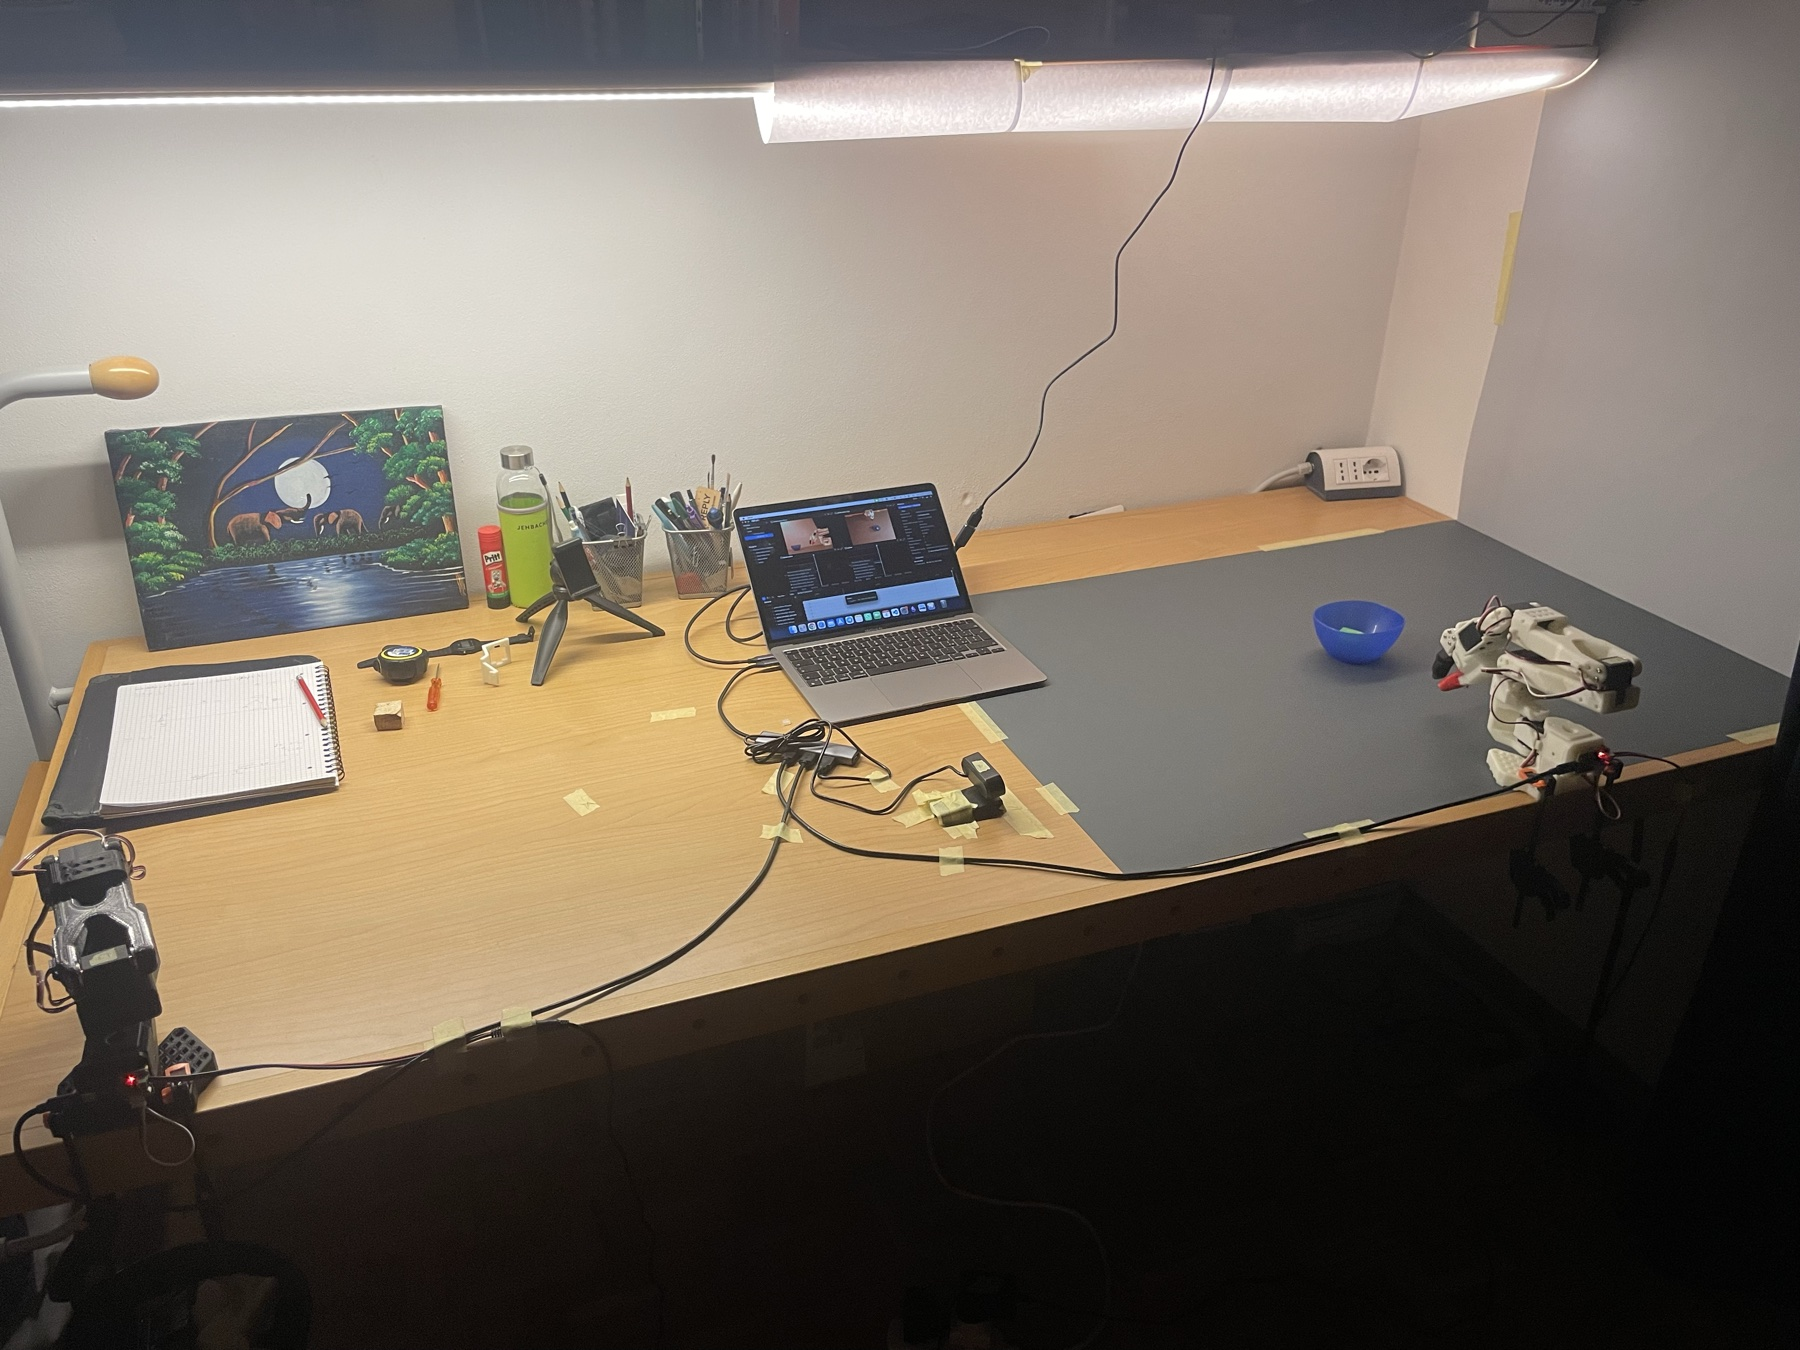
\includegraphics[width=\linewidth]{workspace.jpg}
  \end{minipage}\hfill
  \begin{minipage}[c]{0.49\textwidth}
    \footnotesize
    \begin{tabular}{@{}>{\color{ink2}}l>{\raggedright\arraybackslash}p{0.68\linewidth}@{}}
    \toprule
    Robot      & SO-101 leader--follower pair \\
    Actuators  & 12$\times$ Feetech STS3215 servos \\
               & follower: 6$\times$ 12\,V, 1:345 \\
               & leader: 7.4\,V, 1:345 / 1:191 / 1:145 \\
    Cameras    & 2$\times$ USB webcam, 640$\times$480 @ 30\,fps \\
    Host       & MacBook Air M1 (MPS backend) \\
    Framework  & LeRobot 0.6.2 (\texttt{64b23178}) \\
    Policy     & ACT, 51.6M params, ResNet18 \\
    Training   & NVIDIA T4 (Kaggle / Lightning AI) \\
    \bottomrule
    \end{tabular}
  \end{minipage}
  \caption{The workspace. The leader arm (black, left) is moved by hand to
  teleoperate the follower (white, right); the task is performed on the dark
  mat with the bowl at a fixed, marked position.}
  \label{fig:setup}
\end{figure}

\paragraph{Task.} Pick up a cube from a flat work surface and place it in a
bowl. The bowl is fixed; the cube position is randomised across the workspace
on every episode.

\paragraph{Controls.} Every variable except cube position was held fixed within
a dataset: camera positions marked on the table and never moved; bowl position
marked; constant artificial lighting with blinds closed; fixed arm home
position; matte work surface, taped down and outlined.

\paragraph{Observations.} The policy receives the six joint positions and two
camera streams: an overhead view, which shows the object layout, and a front
view, which shows gripper height. Their placement defines the two camera
setups described next.

% =====================================================================
\section{Datasets, setups and models}
\label{sec:progression}
% =====================================================================

The project went through three iterations. Each was triggered by a specific
failure of the previous one; Table~\ref{tab:progression} maps datasets to
setups and models.

\begin{table}[h]
\centering
\small
\begin{tabular}{@{}llrrll@{}}
\toprule
\textbf{Dataset} & \textbf{Setup} & \textbf{Episodes} & \textbf{Frames} & \textbf{Protocol} & \textbf{Models} \\
\midrule
1 \ \texttt{so101\_cube\_demo\_0} & 2 & 100 & 44{,}553 & original & \texttt{act\_so101\_cube\_100} \\
2 \ \texttt{so101\_cube\_v2}      & 2 & 100 & 47{,}872 & revised  & \texttt{v2\_024}, \texttt{v2\_100} \\
3 \ \texttt{so101\_cube\_v3}      & 3 &  51 & 24{,}404 & revised  & \texttt{v3\_050} \\
\bottomrule
\end{tabular}
\caption{Datasets, camera setups and the models trained on them. All datasets
are recorded at 30\,fps with 16\,s episodes. \texttt{v2\_024} uses episodes
0--23 of dataset~2. Models are referred to by short names throughout:
\texttt{v2\_024}, \texttt{v2\_100} and \texttt{v3\_050} stand for
\texttt{act\_so101\_cube\_v2\_024}, \texttt{act\_so101\_cube\_v2\_100} and
\texttt{act\_so101\_cube\_v3\_050}.}
\label{tab:progression}
\end{table}

\subsection{Iteration 1: the pilot dataset and a gripper that never opened}
\label{sec:gripper}

The first 100 demonstrations were recorded the way a person naturally performs
the task: a quick, loosely controlled reach toward the cube, opening the
gripper only on arrival, closing it, and carrying the cube to the bowl. The
resulting model (\texttt{act\_so101\_cube\_100}) moved toward the cube with a
visibly jittery arm and \textbf{kept the gripper closed}, or almost closed,
throughout. Rather than training longer, the action distribution of the dataset
was examined directly.

The gripper is one of six action dimensions, so under MEAN\_STD normalisation
it contributes one sixth of the loss. Because it opened only in the last
instant before the grasp, 61\% of all frames had it closed and the median
action was 1.2 on a range up to 79 (Figure~\ref{fig:gripper}, left). A policy
that always predicts ``closed'' matches the majority of frames and pays almost
nothing in loss --- while failing at exactly the moment that determines task
success.

\begin{figure}[!h]
  \centering
  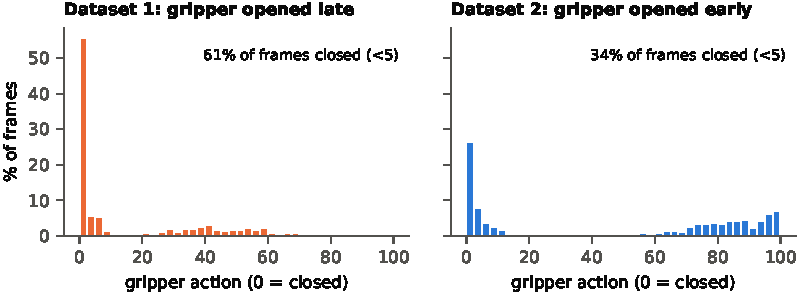
\includegraphics[width=\textwidth]{gripper.pdf}
  \caption{Distribution of the gripper action over all frames. With the
  original protocol (dataset~1, left) the gripper opens only just before the
  grasp and most frames are ``closed''. Opening it at the start of the episode
  (dataset~2, right) moves a large share of frames to the open state.}
  \label{fig:gripper}
\end{figure}

\paragraph{Revised protocol.} Dataset~2 was recorded with slower, deliberate
demonstrations, often with one hand on the leader's trigger and the other
steadying the leader arm, and the gripper opened at the \emph{start} of every
episode: home $\rightarrow$ open gripper fully $\rightarrow$ slow approach
$\rightarrow$ pause above the cube $\rightarrow$ decisive close $\rightarrow$
lift, transport, release above the bowl. Episodes end at release; the return
home happens during the unrecorded reset window. The share of ``closed'' frames
fell from 61\% to 34\%, and every model trained on the revised data opens the
gripper correctly. The lesson generalises: in behaviour cloning a failure mode
can be a property of the \emph{demonstration distribution} rather than of the
model or the training budget, and the dataset is the first place to look.

\subsection{Setup 2: the main dataset}

Datasets~1 and~2 share the same camera arrangement (Figure~\ref{fig:setup2}).
The overhead camera is fixed under the shelf above the desk and looks straight
down on the workspace. The front camera stands on a small tripod at the side
of the table, slightly above the work surface, and looks across it toward the
arm. The effective workspace --- the area in which the cube is placed --- is
about $40\times40$\,cm. The object is a pale yellow cube. Dataset~2 is the main
dataset of the study.

\begin{figure}[!h]
  \centering
  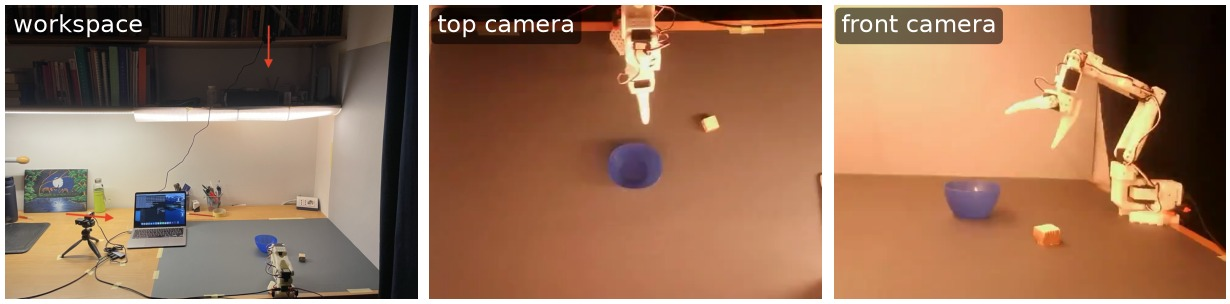
\includegraphics[width=\textwidth]{setup2.jpg}
  \caption{Setup 2. Left: the workspace, with arrows marking where the two
  cameras look. Centre and right: the two observation streams at the resolution
  the policy receives. The cube occupies roughly $30\times30$ pixels and is
  clearly resolved in both views.}
  \label{fig:setup2}
\end{figure}

\subsection{Setup 3: a perceptual redesign}
\label{sec:v3}

The models trained on dataset~2 performed poorly (Section~\ref{sec:results}),
and inspection of their observations suggested a perceptual problem
(Section~\ref{sec:diagnosis}). To test whether better visibility would help,
the scene was redesigned (Figure~\ref{fig:setup3}) and dataset~3 recorded with
the revised protocol:
\begin{enumerate}
  \item a saturated green cube instead of the pale yellow one, which had weak
        contrast against the surface under warm light;
  \item red tape on the gripper tips, a distinct visual reference for the grasp
        point;
  \item the front camera lowered to work-surface level, making gripper height
        legible;
  \item the overhead camera moved to the corner of the shelf and tilted by
        about 30\textdegree{} from the vertical rather than pointing straight
        down, recovering perspective;
\end{enumerate}
Space constraints prevented moving the overhead camera to the side opposite the
arm's entry, so occlusion during the final descent was reduced but not
eliminated.

\begin{figure}[t]
  \centering
  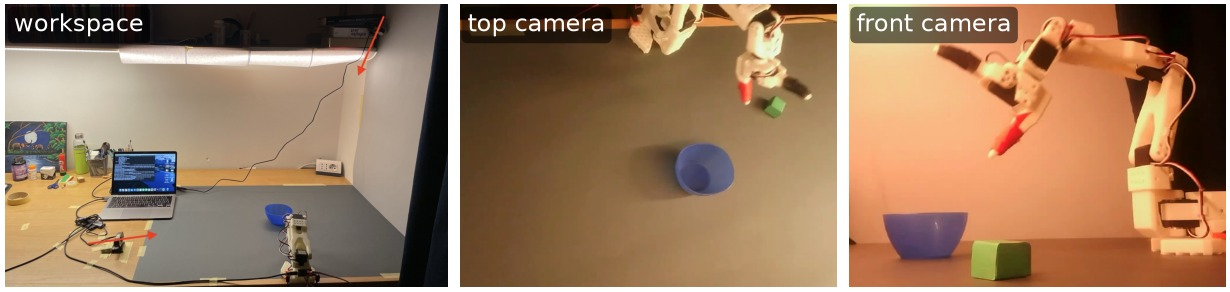
\includegraphics[width=\textwidth]{setup3.jpg}\\[3pt]
  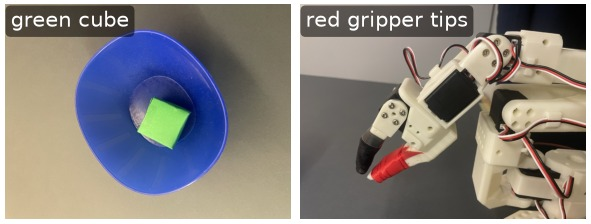
\includegraphics[width=0.48\textwidth]{setup3_details.jpg}
  \caption{Setup 3. Arrows mark where the cameras look: the front camera sits
  at work-surface level and the overhead camera is tilted by about
  30\textdegree{} from the vertical. The green cube and red gripper tips raise contrast in both
  views.}
  \label{fig:setup3}
\end{figure}

% =====================================================================
\section{Training and evaluation protocol}
% =====================================================================

\paragraph{Training.} Identical hyperparameters for the three evaluated models:
ACT with \texttt{chunk\_size}\,=\,\texttt{n\_action\_steps}\,=\,100,
ImageNet-pretrained ResNet18 backbone, AdamW with learning rate $10^{-5}$,
batch size 32, 20{,}000 steps, seed 42. Training cost depends on
steps $\times$ batch size, not on dataset size: with fewer demonstrations the
model simply sees more epochs. The 24 vs.\ 100 comparison is therefore
\emph{data quantity at a fixed optimisation budget} --- the question that
matters to someone deciding how many demonstrations to record. Because the 24
episodes are a nested subset of the 100, it is isolated from lighting drift,
operator fatigue and setup changes; for this to be valid the cube position was
randomised episode by episode across the whole workspace.

\paragraph{Evaluation.} 15 cube positions, marked so that they are visible to
the operator but not to the cameras, identical across all models; a fixed rollout duration of 22\,s for every
model and position; scene conditions identical to data collection. Each rollout is
graded on a four-level scale fixed before evaluation:

\begin{center}
\small
\begin{tabular}{@{}cl>{\raggedright\arraybackslash}p{0.62\textwidth}r@{}}
\toprule
 & \textbf{Outcome} & \textbf{Definition} & \textbf{Points} \\
\midrule
\oa & success      & cube ends in the bowl & 3 \\
\ob & partial      & cube picked up but not deposited in the bowl & 2 \\
\oc & near miss    & correct motion, but the gripper closes within about 1\,cm of the cube & 1 \\
\od & failure      & anything else & 0 \\
\bottomrule
\end{tabular}
\end{center}

The headline metric is the success rate (outcome \textbf{a}), reported with
Wilson 95\% confidence intervals; at $n=15$ these are wide, and reporting them
is the point. The points are a coarse, ordinal summary of \emph{how close} a
model gets to the goal. They are not a calibrated measure and are used only to
compare the three models qualitatively.

% =====================================================================
\section{Results}
\label{sec:results}
% =====================================================================

\begin{table}[t]
\centering
\small
\begin{tabular}{@{}lrrrccr@{}}
\toprule
\textbf{Model} & \textbf{Demos} & \textbf{Epochs} & \textbf{Final $L_1$} & \textbf{Success} & \textbf{95\% CI} & \textbf{Points} \\
\midrule
\texttt{v2\_024} & 24  & 55.7           & 0.050                   & 1/15 \ (6.7\%) & 1--30\% & 13 \\
\texttt{v2\_100} & 100 & 13.4           & 0.076                   & 2/15 (13.3\%)  & 4--38\% & 16 \\
\texttt{v3\_050} & 51  & 19.7$^\dagger$ & $\approx$0.09$^\dagger$ & 2/15 (13.3\%)  & 4--38\% & 18 \\
\bottomrule
\end{tabular}
\caption{Main comparison. Same hyperparameters, same 15 evaluation positions;
points out of 45. $^\dagger$Training of \texttt{v3\_050} stopped at 15{,}000 of
20{,}000 steps because of repeated cloud interruptions.}
\label{tab:main}
\end{table}

\begin{figure}[t]
  \centering
  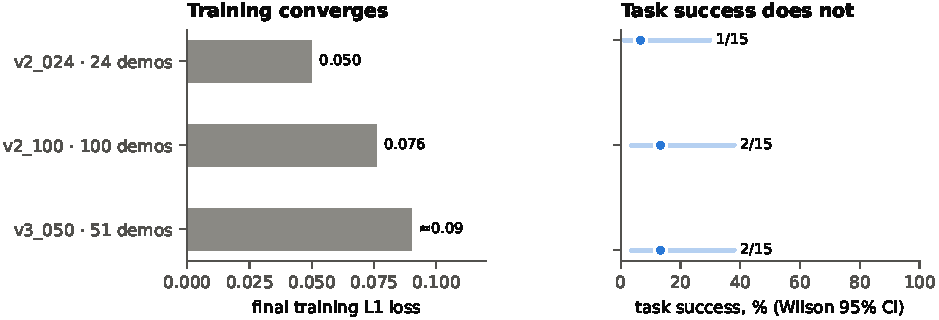
\includegraphics[width=\textwidth]{results.pdf}
  \caption{Every run reduces the $L_1$ loss by an order of magnitude from
  $\approx$0.5--0.6 and flattens (left), yet task success stays low and the
  confidence intervals overlap almost entirely (right).}
  \label{fig:results}
\end{figure}

\paragraph{Training converges.} All runs reduce $L_1$ loss by an order of
magnitude and flatten (Table~\ref{tab:main}, Figure~\ref{fig:results}).
Optimisation is not the limiting factor.

\paragraph{More data does not raise success.} Going from 24 to 100
demonstrations moves success from 1/15 to 2/15, with heavily overlapping
intervals. The correct reading is \textbf{no detectable difference at this
sample size}, not that the larger model is better.

\paragraph{Neither does better visibility.} Setup~3 --- higher-contrast object,
marked gripper tips, repositioned cameras --- also reaches 2/15.

\subsection{Outcomes by position}

\begin{table}[t]
\centering
\small
\setlength{\tabcolsep}{0pt}
\renewcommand{\arraystretch}{1.25}
\begin{tabular}{@{}l@{\hspace{8pt}}*{15}{>{\centering\arraybackslash}p{1.9em}}@{\hspace{8pt}}r@{}}
\toprule
\textbf{Position} & 1 & 2 & 3 & 4 & 5 & 6 & 7 & 8 & 9 & 10 & 11 & 12 & 13 & 14 & 15 & \textbf{Pts} \\
\midrule
\texttt{v2\_024} & \oc & \oc & \oa & \oc & \oc & \oc & \od & \oc & \oc & \oc & \oc & \od & \oc & \od & \od & 13 \\
\texttt{v2\_100} & \oc & \oc & \ob & \oc & \oa & \oa & \od & \oc & \od & \oc & \od & \oc & \oc & \od & \oc & 16 \\
\texttt{v3\_050} & \oa & \oc & \oc & \oc & \oc & \oa & \oc & \oc & \od & \oc & \oc & \oc & \oc & \oc & \oc & 18 \\
\bottomrule
\end{tabular}

\smallskip
{\footnotesize
\colorbox{outA}{\textcolor{white}{\textbf{a}}}~success \quad
\colorbox{outB}{\textcolor{white}{\textbf{b}}}~picked up, not deposited \quad
\colorbox{outC}{c}~near miss ($\lesssim$1\,cm) \quad
\colorbox{outD}{\textcolor{ink2}{d}}~failure \quad
(points: a\,=\,3, b\,=\,2, c\,=\,1, d\,=\,0)}
\caption{Outcome of every evaluation rollout. Each cell is a single rollout at
a fixed, marked cube position.}
\label{tab:positions}
\end{table}

\begin{figure}[t]
  \centering
  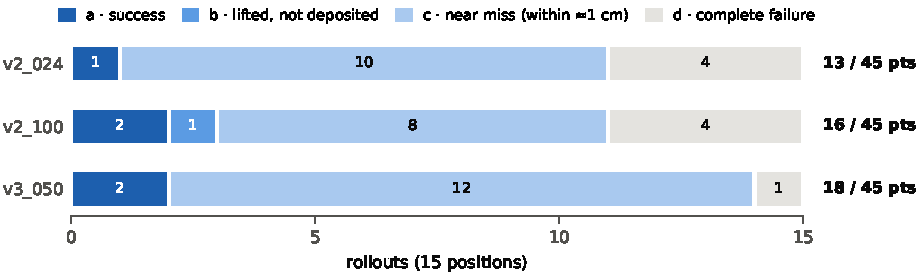
\includegraphics[width=\textwidth]{outcomes.pdf}
  \caption{Outcome distribution per model. Successes stay at 1--2, but the share
  of complete failures falls from 4 to 1 with setup~3, and nearly every rollout
  of \texttt{v3\_050} ends at least in a near miss.}
  \label{fig:outcomes}
\end{figure}

Table~\ref{tab:positions} and Figure~\ref{fig:outcomes} show what the success
rate hides.

\paragraph{The dominant outcome is a near miss.} 10, 8 and 12 of the 15
rollouts of the three models end with the gripper closing within about a
centimetre of the cube (Figure~\ref{fig:teaser}, bottom). The arm lifts, moves
to the correct region and opens and closes the gripper in the right order; it
fails only in the final alignment.

\paragraph{A qualitative progression.} Points rise from 13 to 16 to 18. The
largest change is not in successes but in complete failures, which drop from 4
(both setup-2 models) to 1 with setup~3: positions 7 and 14, total failures
for both setup-2 models, become near misses. With $n=15$ this difference is
not statistically significant (Fisher's exact test, $p=0.33$), so it is an
indication rather than a result --- but it points in the same direction as
the qualitative observations below.

\paragraph{Qualitative observations from the evaluation.}
\begin{itemize}
  \item \texttt{v3\_050} is generally better at \emph{second attempts}: after a
        missed grasp it reacts faster and its retry is more accurate.
  \item Outcomes are not deterministic. A success at a given position does not
        mean the same position succeeds again; each cell in
        Table~\ref{tab:positions} is one sample.
  \item The policies do not follow the bowl if it is moved: they release at the
        place where the bowl usually is. Since the bowl was fixed in every
        demonstration, the transport phase is tied to a coordinate in the
        workspace rather than to the bowl as an object.
\end{itemize}

% =====================================================================
\section{What the policy did learn}
\label{sec:learned}
% =====================================================================

A 7--13\% success rate could suggest a policy that has learned little. The
rollouts show otherwise. Every evaluated model reproduces the full structure of
the task --- approach, open, descend, close, lift, transport, release --- and
aims at the correct region of the workspace for each cube position. The
failures are concentrated in the last centimetre.

More tellingly, the policies \textbf{react to the outcome of their own grasp}.
In additional, informal rollouts with longer durations (30, 40 and 50\,s), a missed
grasp is often followed by a characteristic sequence: the arm starts moving
toward the bowl with an empty gripper, then turns back, returns to the cube and
tries again. Figure~\ref{fig:retry} shows a single, uninterrupted rollout of
\texttt{v3\_050} in which the first grasp misses, the arm leaves, comes back,
regrasps and completes the task.

\begin{figure}[h]
  \centering
  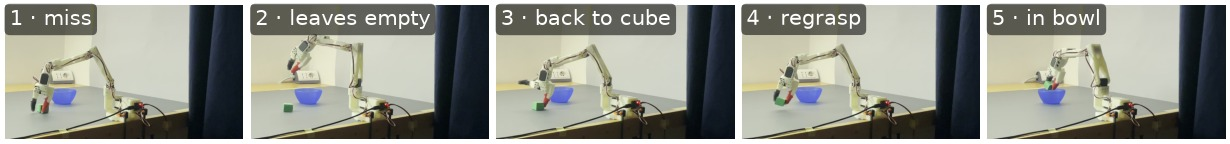
\includegraphics[width=\textwidth]{retry.jpg}
  \caption{One continuous rollout of \texttt{v3\_050}: the first grasp misses
  (1), the arm starts toward the bowl with an empty gripper (2), returns to the
  cube (3), regrasps (4) and deposits it (5). Video in Section~\ref{sec:videos}.}
  \label{fig:retry}
\end{figure}

This behaviour was never demonstrated: every training episode contains exactly
one, successful grasp. It means the policy uses its observations to tell
whether the cube is in the gripper and where it roughly lies, and re-plans
accordingly. The delay before it turns back is consistent with action chunking:
with \texttt{n\_action\_steps}\,=\,100 the policy executes about 3.3\,s of
actions before observing the scene again, so it commits to the transport
motion before it can notice the miss.

The picture is therefore not of a policy that ignores vision, but of one that
extracts \emph{coarse} information --- task phase, grasp success, approximate
cube location --- and lacks the \emph{fine} information needed to close the
last centimetre. That is precisely what the camera geometry predicts.

% =====================================================================
\section{Diagnosis: a perceptual bottleneck}
\label{sec:diagnosis}
% =====================================================================

\paragraph{Low loss with poor performance is the key observation.} A low $L_1$
means the policy accurately predicts the \emph{demonstrated} actions. If the
exact object position were usable from the observations, conditioning on it
would lower the loss further --- a trajectory aimed at the actual cube matches
each demonstration better than an approximate one. The policy does not get
there, which suggests the fine-grained information is not reaching the model
in a usable form.

\paragraph{It is not resolution.} The first hypothesis --- that the cube is too
small in the input images --- was tested by inspecting dataset frames at the
resolution the policy receives. The cube is clearly resolved in both views
(Figure~\ref{fig:setup2}).

\paragraph{It is geometry.} What is missing is not the object but the
\emph{relative} position of gripper and object at the moment that matters
(Figure~\ref{fig:bottleneck}). In the overhead view the arm enters from the
frame edge and occludes the grasp region as the gripper descends. In the front
view gripper height is legible, but depth along the viewing axis is ambiguous.
At the instant of closure neither view gives a reliable estimate of the
gripper--object alignment error, so the policy has no signal to correct the
last centimetre from.

\begin{figure}[!h]
  \centering
  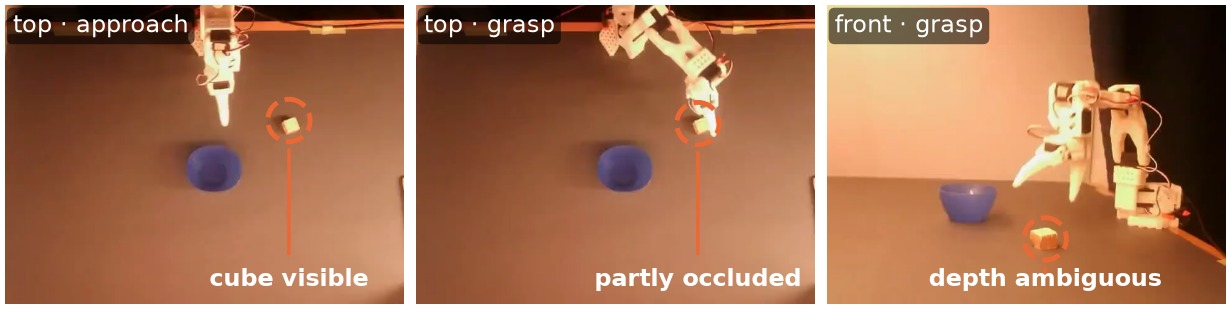
\includegraphics[width=\textwidth]{bottleneck.jpg}
  \caption{The same setup-2 demonstration seen by the policy. During the
  approach the cube is clearly visible from above (left). At the grasp, the arm
  covers it in the overhead view (centre), while the front view cannot resolve
  whether the gripper is in front of or behind it (right).}
  \label{fig:bottleneck}
\end{figure}

\paragraph{What setup 3 changed, and what it did not.} Better contrast and
camera angles did not raise the success rate, but they may have reduced
complete failures and improved retries (Section~\ref{sec:results}). This is
what a geometric bottleneck predicts: improved visibility helps the
\emph{coarse} stages --- finding the cube, recognising a miss --- while the
final alignment, which depends on seeing gripper and cube together, is
unchanged.

\subsection{Converging evidence}

\begin{enumerate}
  \item Training loss is low and flat $\rightarrow$ optimisation is not limiting.
  \item 4$\times$ more data does not change the success rate $\rightarrow$
        sample count is not limiting.
  \item Most failures are near misses, and the policy retries after a miss
        $\rightarrow$ task structure and coarse localisation are learned.
  \item Better contrast and camera angles do not change the success rate
        $\rightarrow$ object \emph{visibility} is not limiting.
\end{enumerate}
What remains is the geometry of what the cameras see at the critical moment.

\paragraph{The implied fix.} A \textbf{wrist-mounted camera} observes gripper
and object together, without occlusion, throughout approach and grasp --- which
is why most manipulation setups include one. It was omitted early in this
project for a deformable-object task (where the cloth is occluded by the
gripper during grasping) that was later dropped, and the decision was not
revisited when the scope changed. Without a 3D printer no adequate mount could
be made, and by the time of the diagnosis there was no time to re-record a full
dataset. It is the primary next step, and it is motivated by the collected data
rather than by general practice.

% =====================================================================
\section{Limitations and scope}
\label{sec:scope}
% =====================================================================

\begin{itemize}
  \item \textbf{Sample size.} 15 rollouts per model give wide intervals;
        differences smaller than roughly 25 percentage points in success rate
        are not detectable.
  \item \textbf{One rollout per position.} Outcomes are not deterministic, so
        per-position results are single samples, not position-level
        properties.
  \item \textbf{Ordinal scoring.} The points scale summarises the outcome
        distribution; it is not a calibrated measure of performance.
  \item \textbf{Two data points, not a curve.} The planned 10/25/50/100 sweep
        was reduced to 24/100.
  \item \textbf{No out-of-distribution evaluation.} With in-distribution
        success at 7--13\%, OOD evaluation would have produced 0--1 successes
        out of 15; it was omitted deliberately. The bowl observation in
        Section~\ref{sec:results} is anecdotal.
  \item \textbf{Setup 3 is not a controlled ablation.} Four changes were
        applied together to maximise the chance of a detectable effect, and
        \texttt{v3\_050} training stopped at 15{,}000 steps.
  \item \textbf{Single operator.} Demonstration quality was not independently
        assessed.
  \item \textbf{Mechanical repeatability.} The SO-101 uses 3D-printed PLA parts
        with gearbox backlash; sub-centimetre repeatability was not
        characterised and may contribute to the near misses.
\end{itemize}

\paragraph{Scope management.} The plan was reduced three times, each time
deliberately, to guarantee a finished project. Each reduction kept the central
question and removed what was redundant or not measurable in the available
time.

\begin{center}
\small
\begin{tabular}{@{}lll@{}}
\toprule
 & \textbf{Original plan} & \textbf{Delivered} \\
\midrule
Tasks & rigid cube $+$ deformable cloth & cube only \\
Data levels & 10 / 25 / 50 / 100 & 24 / 100 \\
Rollouts per condition & 25 & 15 \\
OOD factors & position, colour, size, target & none \\
Total rollouts & 320 & 45 \\
\bottomrule
\end{tabular}
\end{center}

% =====================================================================
\section{Conclusion and future work}
% =====================================================================

The policies trained here succeed on 7--13\% of attempts. Four times more data
does not raise that rate, and neither does a redesigned, higher-contrast
perceptual setup, while training loss converges cleanly in every case. The
policies are nonetheless competent at everything except the last centimetre:
they reproduce the task structure, aim at the right place, and recover from a
missed grasp. Together these locate the limitation: the relative alignment of
gripper and object at the moment of grasping is not visible in either camera
view when it is needed.

The practical lesson is that camera placement deserves at least as much
attention as dataset size, and that for precise manipulation a wrist camera is
a structural requirement, not an optional refinement. The methodological lesson
is that training loss and task success can diverge sharply in behaviour
cloning, that a binary success rate hides much of what a policy has learned,
and that the gap between them is where the useful diagnostic information lives.

\paragraph{Next steps.} In order of expected impact:
\begin{enumerate}
  \item \textbf{Wrist camera} --- directly addresses the identified bottleneck.
  \item \textbf{Varying the bowl position} in the demonstrations, so that
        placement is conditioned on the bowl rather than on a coordinate.
  \item \textbf{Reduced workspace} --- higher demonstration density for the same
        episode count.
  \item \textbf{Non-learning baseline} --- OpenCV cube detection plus inverse
        kinematics, to bound the task and isolate the contribution of learning.
  \item \textbf{Pre-trained policies} (SmolVLA, $\pi_0$) fine-tuned on the same
        data, starting from far richer visual representations.
  \item \textbf{OOD evaluation}, once in-distribution performance is high enough
        for it to be informative.
\end{enumerate}

% =====================================================================
\section*{Videos}
\label{sec:videos}
% =====================================================================

\begin{center}
\videocard{thumb_teleop.jpg}{Teleoperation}{\urlOverview}\hfill
\videocard{thumb_success.jpg}{Successful rollout}{\urlSuccess}\hfill
\videocard{thumb_failure.jpg}{Near miss}{\urlFailure}\hfill
\videocard{thumb_retry.jpg}{Miss, retry, success}{\urlRetry}
\end{center}

\paragraph{Acknowledgements.} Built on the open-source SO-100/SO-101 design by
TheRobotStudio and the LeRobot framework by Hugging Face.

% =====================================================================
\appendix
\clearpage
\section{Reproducing this work}
% =====================================================================

\paragraph{Published artifacts.}
\begin{center}
\small
\begin{tabular}{@{}ll@{}}
\toprule
\textbf{Artifact} & \textbf{Identifier} \\
\midrule
Dataset 1, pilot (setup 2) & \href{https://huggingface.co/datasets/Fabyo04/so101_cube_demo_0_20260926_155239}{\texttt{Fabyo04/so101\_cube\_demo\_0\_20260926\_155239}} \\
Dataset 2, main (setup 2) & \href{https://huggingface.co/datasets/Fabyo04/so101_cube_v2}{\texttt{Fabyo04/so101\_cube\_v2}} \\
Dataset 3 (setup 3) & \href{https://huggingface.co/datasets/Fabyo04/so101_cube_v3}{\texttt{Fabyo04/so101\_cube\_v3}} \\
Model, dataset 1 & \href{https://huggingface.co/Fabyo04/act_so101_cube_100}{\texttt{Fabyo04/act\_so101\_cube\_100}} \\
Model, dataset 2, 24 demos & \href{https://huggingface.co/Fabyo04/act_so101_cube_v2_024}{\texttt{Fabyo04/act\_so101\_cube\_v2\_024}} \\
Model, dataset 2, 100 demos & \href{https://huggingface.co/Fabyo04/act_so101_cube_v2_100}{\texttt{Fabyo04/act\_so101\_cube\_v2\_100}} \\
Model, dataset 3 & \href{https://huggingface.co/Fabyo04/act_so101_cube_v3_050}{\texttt{Fabyo04/act\_so101\_cube\_v3\_050}} \\
Code & \linkor{\urlRepo}{GitHub repository} \\
\bottomrule
\end{tabular}
\end{center}

\paragraph{Environment.} LeRobot 0.6.2, commit
\texttt{64b23178d5348609c266250d3e1f511eba4c33ff}; Python 3.12.13; PyTorch
2.11.0. Data collection and inference on macOS arm64 (MacBook Air M1), training
on Linux with an NVIDIA T4. LeRobot evolves rapidly, so the commit hash is
recorded; results are not expected to reproduce exactly across versions. A
secondary training run used LeRobot 0.6.1 on a different platform.

\paragraph{Figures.} Every figure in this report is generated by
\texttt{scripts/make\_report\_figures.py} from the public datasets, the
evaluation sheet (\texttt{Report/Evaluation results.xlsx}) and the photos and
video stills in \texttt{Report/media/}. The stills were extracted once from the
original recordings, which are not published, by
\texttt{scripts/extract\_media\_stills.py}.

\medskip\noindent\textbf{Data collection.}\par
\begin{lstlisting}
lerobot-record \
  --robot.type=so101_follower --robot.port=$FOLLOWER_PORT --robot.id=follower_01 \
  --robot.cameras="{ top: {type: opencv, index_or_path: 0, width: 640, height: 480, fps: 30}, \
                     front: {type: opencv, index_or_path: 1, width: 640, height: 480, fps: 30} }" \
  --teleop.type=so101_leader --teleop.port=$LEADER_PORT --teleop.id=leader_01 \
  --dataset.repo_id=$HF_USER/so101_cube_v2 --dataset.root=$DATASET_ROOT \
  --dataset.num_episodes=25 --dataset.no_stamp=true \
  --dataset.episode_time_s=16 --dataset.reset_time_s=10 \
  --dataset.streaming_encoding=true --dataset.encoder_threads=2 \
  --dataset.rgb_encoder.vcodec=auto \
  --dataset.single_task="Pick up the cube and place it in the bowl"
\end{lstlisting}

\medskip\noindent\textbf{Training.}\par
\begin{lstlisting}
python -m lerobot.scripts.lerobot_train \
  --dataset.repo_id=Fabyo04/so101_cube_v2 \
  --policy.type=act --policy.repo_id=Fabyo04/act_so101_cube_v2_100 \
  --policy.device=cuda \
  --output_dir=outputs/train/act_cube_v2_100 --job_name=act_cube_v2_100 \
  --steps=20000 --batch_size=32 --seed=42 \
  --save_freq=5000 --save_checkpoint_to_hub=true --wandb.enable=false
\end{lstlisting}

\medskip\noindent\textbf{Autonomous rollout.}\par
\begin{lstlisting}
lerobot-rollout \
  --robot.type=so101_follower --robot.port=$FOLLOWER_PORT --robot.id=follower_01 \
  --robot.cameras="{ top: {...}, front: {...} }" \
  --policy.path=Fabyo04/act_so101_cube_v2_100 \
  --policy.n_action_steps=100 \
  --device=mps --fps=30 \
  --task="Pick up the cube and place it in the bowl" --duration=22
\end{lstlisting}

% =====================================================================
\section{Practical notes for building this setup}
% =====================================================================

Things that cost time and are not in the official guides.

\paragraph{Motor variants are visually identical.} The kit contains four
different servos (7.4\,V at three gear ratios for the leader, 12\,V 1:345 for
the follower). Label every motor before assembly. For a spare, the follower's
12\,V unit is the right choice: all six follower joints use the same part, and
the leader --- moved by hand --- rarely fails. One vendor datasheet labels the
12\,V part ``used on leader arm''; this is a copy-paste error. Torque in the
product name is the reliable discriminator: 19\,kg $=$ 7.4\,V $=$ leader,
30\,kg $=$ 12\,V $=$ follower.

\paragraph{Set motor IDs one at a time, before assembly.} Servos ship with
identical IDs on a shared serial bus. During \texttt{lerobot-setup-motors},
disconnect the \emph{DC power}, never the USB --- the USB carries the serial
port, and unplugging it kills the script with
\texttt{termios.error: Device not configured}.

\paragraph{Calibration can silently fail.} A joint reporting a range of 0--4095
has wrapped around the 12-bit encoder boundary, not discovered a
360\textdegree{} joint. Centre every joint in its mechanical travel before the
first prompt, then move one joint at a time. Valid ranges stay well clear of
both 0 and 4095, and leader/follower amplitudes should match.

\paragraph{A motor that stops responding is usually in protection.}
Power-cycle first. One silent motor suggests a connector; six silent motors
suggest upstream power or USB.

\paragraph{Connectors are the weak point.} Three independent
intermittent-contact failures occurred during this project (DC barrel jack,
camera USB cable, leader board USB). Anchor every cable to the table about
10\,cm from its connector before starting, not after the third failure.

\paragraph{Check barrel jack dimensions.} 5.5$\times$2.1\,mm and
5.5$\times$2.5\,mm have identical outer diameters. A mismatch feels like
``needs more force'' and will damage the centre pin if forced.

\paragraph{The frame-rate warning is misleading.} LeRobot's
\textit{``Record loop is running slower''} message is emitted only on slow
iterations and never reports the mean. With ACT's action chunking, one
iteration in a hundred runs full inference and is legitimately slow. Check the
frame count in the \texttt{Map:} line instead, which should approach
\texttt{episode\_time\_s} $\times$ \texttt{fps}.

\paragraph{Enable streaming encoding.} Without
\texttt{--dataset.streaming\_encoding=true --dataset.rgb\_encoder.vcodec=auto},
video encoding competes with the recording loop. With it, per-episode cycle
time dropped from $\approx$65\,s to $\approx$20\,s --- the difference between
35 minutes and two hours for 100 demonstrations. Also disable \texttt{rerun}
visualisation while recording.

\paragraph{macOS specifics.} Serial ports appear as
\texttt{/dev/tty.usbmodem<SERIAL>} and are stable across reboots --- no udev
rules needed. Conversely, \texttt{v4l2-ctl} does not exist and the AVFoundation
backend generally ignores exposure and white-balance settings; control the
lighting instead.

\paragraph{Test the full pipeline on five episodes first.} Record, train
briefly, and run inference end-to-end before committing to a hundred
demonstrations.

\end{document}
